\chapter{Stato dell'arte}
Il mondo mobile fa sempre pi\`u parte della nostra vita e ogni giorno vengono inventate sempre nuove applicazioni che permettono di semplificarla. Esistono app
per poter ascoltare la musica, altre per poter eseguire delle transazioni bancarie ed altre ancora destinate alle domotica, per fare alcuni esempi.

Dato che siamo influenzati cos\`i tanto dal mondo mobile, viene spontaneo chiedersi quali sono le possibili strade da seguire per poter sviluppare un'app.
Innanzitutto \`e necessario fare una distinzione tra app nativa e app multipiattaforma.
Le prime sono delle applicazioni software che sono state sviluppate per funzionare su uno
specifico tipo di dispositivo o piattaforma. Invece la seconda \`e un applicazione che pu\`o essere eseguita anche su sistemi operativi differenti ma usando sempre lo stesso codice.
In particolare un app nativa sviluppata per un dispositivo Android non funzionar\`a su dispositivi iOS e viceversa un app sviluppata
per un dispositivo iOS non funzioner\`a su dispositivi Android \cite{ReactNativeCLI:Expo} \cite{app:ibride:native}.\\

%\section{Sviluppo mobile}
\section{App Multipiattaforma}
React native \`e un Framework per lo sviluppo di app multipiattaforma che permette di sviluppare applicazioni sia per Android che iOS.
Per poter utilizzare questo Framework esistono due principali ``strumenti": Expo\cite{ReactNativeCLI:Expo} e React Native CLI\cite{ReactNativeCLI:Expo}.
Entrambi mettono a disposizione una serie di servizi per aiutare nello sviluppo. In particolare Expo \`e un Framework che estende React Native
\subsection{React Native}
\begin{figure}[h]
      \centering
      
\includegraphics[width=5cm, height=4cm]{images/ReactNativeLogo-NoBackground.png}
      \caption[differenzeiteot]{}
      \label{fig:ReactNative}
\end{figure}

In React Native, proprio come in React, vengono costruiti dei componenti JSX, i quali combinano markup e il JavaScript, che lo controlla, in un unico file. A differenza del web non
si ha una separazione tra grafica, presentazione e controllo in file diversi, in quanto JSX privilegia la separazione delle ``concern" rispetto alla
separazione delle tecnologie.

Il ciclo di aggiornamento \`e lo stesso di React: quando le "props"  o gli "state" cambiano, React Native esegue un nuovo rendering delle viste.\\
La differenza principale tra React Native e React nel browser \`e che React Native sfrutta le librerie dell'interfaccia utente, della sua piattaforma ospitante,
anzich\`e utilizzare il markup HTML e CSS.

React Native CLI permette di utilizzare React Native per sviluppare diversi tipi di applicazioni, tra cui:
\begin{itemize}
      \item Prototipi
      \item Applicazioni multipiattaforma
      \item Applicazioni che non fanno largo uso di API native
      \item Applicazioni con una complessa User Interface {}(UI)
      \item Applicazioni per un determinato sistema operativo
      \item Applicazioni che non fanno uso intensivo di animazioni
\end{itemize}
Tra i vari vantaggi derivanti dall'utilizzo di questo ``strumento", bisogna sottolineare che:
\begin{list}{*}{}
      \item Permette di includere moduli nativi scritti in Java, Kotlin e Object-C
      \item Consente di ridurre i tempi di sviluppo, in quanto permette di riutilizzare gran parte del codice scritto per le applicazioni web
      \item Mette a disposizione un gran numero di componenti pre-costruiti
      \item Fornisce un interfaccia utente semplice
      \item Permette di utilizzare plugin di terze parti
      \item Consente di realizzare una migliore User Interface rispetto ad Expo
      \item Presenta un architettura modulare la quale consente di semplificare lo sviluppo, il test e la manutenzione di programmi di grosse dimensioni
\end{list}
Mentre tra i vari svantaggi, si ha che:
\begin{list}{*}{}
      \item Per poter effettuare i test \`e necessario collegare il dispositivo al Pc
      \item Richiede Android Studio e XCode per l'esecuzione dei progetti
      \item Per poter condividere la propria app \`e necessario condividere l'intero file .apk
      \item La preparazione di un progetto richiedere tempo e non \`e cos\`i  semplice come con Expo
      \item Richiede una conoscenza preliminare della strutturazione delle cartelle in Android e iOS
\end{list}

Una volta installata un'applicazione sviluppata in React Native sul proprio dispositivo, questa non eseguir\`a il render nel browser DOM, anzi andr\`a ad invocare le Object-C APIs, per eseguire il render su dispositivi IOS,
e andr\`a ad invocare le Java APIs, per eseguire il render su dispositivi Android. L'utilizzo di tali API \`e possibile grazie al ``bridge", il quale fornisce a React un'interfaccia con gli elementi
della UI nativa della piattaforma ospitante.\\ In particolare i "React component" restituiscono il markup della loro funzione di rendering,
il quale descrive il loro aspetto. Quando si utilizza React, per lo sviluppo web, questo si traduce direttamente nel DOM del broswer. Per React Native, il markup di un componente viene tradotto per adattarsi alla piattaforma host.
Quindi una $<$View$>$ potrebbe diventare una UIView specifica per iOS \cite{ReactNative} \cite{ReactNativeCLI:Expo}.

\begin{figure}[h]
      \centering
      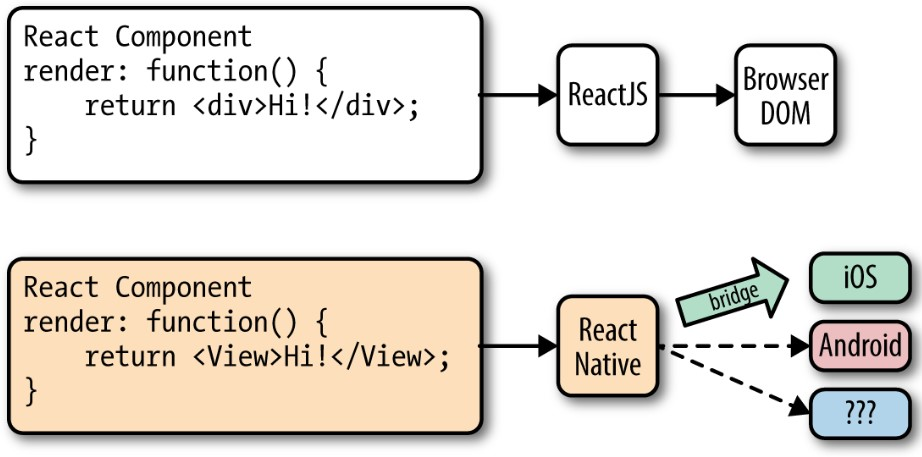
\includegraphics[width=10cm, height=4cm]{images/ReactRendering.jpg}
      \caption[differenzeiteot]{}
      \label{fig:ReactRendering}
\end{figure}


\subsection{Expo}
Expo \`e simile a React Native CLI, ma con uno svantaggio considerevole. In alcune applicazioni \`e necessario
accedere alle API native che non sono disponibili su Javascript, per esempio le API per accedere ad Apple e Google play.
In altri casi all'interno di un'applicazione si
potrebbe voler riutilizzare le librerie scritte in Java, Object-C,Swift,Kotling o C++ che non sono state implementate in Javascript.

I moduli nativi permettono di esporre
delle istanze di classi Java, Object-C e C++ come oggetti JavaScript. In questo modo \`e possibile eseguire codice nativo in JavaScript.\\
Expo non permette di utilizzare i moduli nativi, quindi a meno che una certa libreria non sia gi\`a stata implementata in JavaScript, questa non potr\`a essere utilizzata
in un'applicazione sviluppata tramite Expo.
Questo non \`e l'unico svantaggio derivante dall'utilizzo di questo strumento. Alcune device API non sono supportate, come ad esempio il bluetooth.\\
A parte questo Expo presenta diversi vantaggi, tra cui \cite{ReactNative:Sito} \cite{ReactNativeCLI:Expo}:
\begin{list}{*}{}
      \item Una migliore gestione dei link
      \item Mette a disposizione una maggiore quantit\`a di librerie standart, come ad esempio una libreria per le "Push Notification"
      \item Offre una migliore "Development Experience". Per poter testare un'applicazione, sviluppata tramite Expo, non \`e necessario avere un emulatore del dispositivo, su cui la si vuole testare, o collegare il proprio dispositivo al pc
            Expo permette di testare le applicazioni tramite Wi-fi, collegando il dispositivo e il pc alla stessa rete LAN
      \item Le applicazioni vengono aggiornate pi\`u velocemente rispetto a React Native CLI
      \item Supporta "l'Over to air update", quindi un applicazione si aggiorna nel momento in cui quest'ultima si sta aprendo sul dispositivo su cui \`e installata
      \item Non \`e necessario effettuare la build dell'applicazione per poterla testare
      \item \`E possibile "espellere" il progetto in ExpoKit e integrare del codice nativo, continuando ad utilizzare alcune funzionalit\`a di Expo, ma non tutte
\end{list}

\subsection{React Navigation}
Sia che si utilizzi Expo o React Native CLI, aspetti molto importanti nello sviluppo di un'app sono la presentazione e la navigazione tra i vari ``Screen". Quest'ultimi
rappresentano la parte di User Interface con la quale l'utente interagir\`a. La navigazione tra i vari screen
viene gestita da un ``Navigator". Il principale Navigator utilizzato sia da Expo che da React Native si chiama ``React Navigation".
Questa \`e una standalone library che permette di gestire lo spostamento tra i vari screen di cui l'applicazione \`e composta.

React Navigation fornisce principalmente quattro Navigator\cite{ReactNavigation}, ognuno dei quali consente ad un utente di passare da uno screen ad un altro:
\begin{itemize}
      \item Native Stack Navigator: Ogni volta che un utente effettua una transizione
            il nuovo screen viene messo in cima allo stack. Il Native Stack Navigator utilizza le API native UINavigationController per le applicazione sviluppate per iOS e le API native Fragment per le
            applicazioni sviluppate per Android. \\In questo modo la navigazione tra i vari screen avr\`a lo stesso comportamento e le stesse prestazioni
            di applicazioni che usano la navigazione nativa. Nonostante le prestazioni fornite da questo Navigator siano ottime, non \`e particolarmente "customizzabile"
            come lo Stack Navigator.
      \item Stack Navigator: A differenza del Native Stack Navigator questo \`e incredilmente "customizzabile", poich\`e implementato in Javascript. Nonostante ci\`o non usando le primitive di navigazione native
            presenta prestazioni peggiori. Va comunque detto che per la maggior parte delle applicazioni questa differenza di performance tra il Native Stack Navigator e lo Stack Navigator non \`e percebile.
      \item Drawer Navigator: La differenza principale tra questo Navigator e gli altri \`e che quest'ultimo viene rappresentato con un icona formato da tre linee orizzontali, posta in alto a sinistra della visualizzazione. Attraverso
            quest'ultima \`e possibile vedere tutti gli screen su cui si pu\`o navigare.
      \item Tab Navigator: Questo Navigator viene rappresentato tramite una Tab-Bar posta nella parte bassa dello schermo. Essa mostra gli screen verso cui si
            pu\`o navigare. Questo Navigator \`e uno dei pi\`u utilizzati nelle applicazioni basate su Tab-Bar.
\end{itemize}


\subsection{Redux}

Al giorno d'oggi le single-page application devono gestire sempre pi\`u stati, ed \`e per questo che nella maggior parte delle app
si utilizza Redux. Questa \`e una libreria molto leggera che aiuta a sviluppare applicazioni che si comportano in modo coerente, che vengono eseguite in
ambienti diversi (client e server) e che sono facili da testare. Si dice che Redux permetta di realizzare un ``contenitore a stato" prevedibile, per le applicazioni JavasScript.

Questa libreria \`e completamente compatibile con React Native, attraverso l'utilizzo di React Redux, il quale rappresenta il livello di binding ufficiale di React UI per Redux.
Questo livello consente ai "React component" di leggere i dati da un archivio e di inviare azioni a quest'ultimo per aggiornarne lo stato.\\
In particolare, Redux:
\begin{itemize}
      \item Permette di realizzare uno store che contiene lo stato globale
      \item Consente di emettere azioni che aggiornano lo stato dello store. Queste vengono notificate all'archivio nel momento in cui avviene un evento nell'applicazione
      \item Presenta delle funzioni riduttrici pure che esaminano le azioni e restituiscono uno stato immutabile aggiornato
\end{itemize}
Quando si parla di ``stati" da gestire all'interno di un'app, si fa riferimento, ad esempio: alle risposte di un server, a dati salvati nella
cache o creati locamente e che non sono memorizzati in modo persistente. Redux \`e in grado di gestire tutti questi stati e permette di rendere la mutazione
dello stato globale prevedibile, attraverso l'imposizione di alcune restrizioni, su quando e come lo stato pu\`o essere modificato.

Queste restrizioni possono essere riassunte nei tre principi cardine di Redux\cite{Redux}:

\begin{enumerate}
      \item Lo stato globale dell'applicazione \`e memorizzato in un albero di oggetti all'interno di un singolo store. In questo modo \`e possibile realizzare app universali, permettere un miglior debugging dell'applicazione e
            rendere lo stato globale persistente in modo da avere un ciclo di sviluppo pi\`u rapido.
      \item Lo stato \`e Read Only. Questo assicura che n\'e le ``viste" n\'e le callback di rete scrivano direttamente sullo stato. Al contrario, esprimono l'intenzione di trasformare lo stato.
            \\Dato che tutte le modifiche sono centralizzate e avvengono una alla volta in un ordine rigoroso, non vi sono condizioni di concorrenza a cui dover prestare attenzione.
            Le azioni per aggiornare lo stato sono semplici oggetti JavaScript, quindi possono essere registrate, serializzate, memorizzate e successivamente riprodotte per scopi
            di debug o di test.
      \item Lo stato viene aggiornato da funzioni pure, le quali sono chiamate riduttori. Queste prendono lo stato precendete, un'azione e restituiscono lo stato successivo.
            In particolare i riduttori devono ritornare nuovi oggetti di stato e non modificare lo stato precendente.

\end{enumerate}

%\subsubsection{React Native}
%\subsubsection{Expo}
\section{App Native}

Come gi\`a menzionato all'inizio di questo capitolo, le applicazioni native sono sviluppate per uno specifico dispositivo o piattaforma ed \`e quindi necessario un linguaggio di programmazione differente da un sistema operativo all'altro.
iOS fa uso dei linguaggi Object-C e Swift, mentre Android sviluppa app native in Java e Kotlin.
\subsection{Kotlin}

Kotlin \`e un linguaggio sviluppato da JetBrains a partire dal 2010 e successivamente reso open source nel 2012. \`E definito come general purpose, free, open source e pragmatico. Pragmatico in quanto cerca di distinguersi dalla struttura chiusa e ben
definita di Java al fine di permettere uno sviluppo pi\`u snello e veloce, grazie soprattutto al fatto che fornisce diversi ``shortcut".

Koltin nel 2019 \`e diventato, secondo Google, il linguaggio pi\`u utilizzato per lo sviluppo di applicazioni Android, sostituendo Java \cite{KotlinTech}.
Nonostante lo si utilizzi per lo sviluppo di applicazioni Android native, quest'ultimo permette anche la realizzazione di applicazioni per iOS e di applicazioni web, in quanto \`e possibile transpilare il codice scritto in Kotlin
in codice JavaScript \cite{Kotlin:JetBrains}.
%Oltre ad essere utilizzato per lo sviluppo front-end, quindi lato client, pu\`o essere utilizzato anche per lo sviluppo backend. In particolare Kotlin pu\`o lavorare con diverse tecnologie lato server, come WebGL o Node.js.\\

Kotlin consente di realizzare applicazioni seguendo il paradigma Object Oriented {}(OOP) o il paradima della programmazione funzionale. Nel primo caso si fa uso delle classi, dell'ereditariet\`a e del polimorfismo, proprio come in Java.
Nel secondo caso il programma si basa sulla valutazione di funzioni matematiche. In questo modo \`e possibile ottenere il meglio dei due mondi\cite{KotlinInfoWorld}.

Un ambiente di esecuzione per le applicazioni scritte tramite questo linguaggio, \`e la JVM {}(Java Virtual Machine). Questo ambiente di esecuzione consente di utilizzare Kotlin in
qualsiasi contesto in cui viene utilizzato Java. Inoltre, Kotlin \`e al 100\% interoperabile con quest'ultimo. Il vantaggio di questo alto livello di interoperabilt\`a \`e che si possono riutilizzare le librerie Java esistenti\cite{kotlin}.

Kotlin e Java sono molto simili tra loro, ed entrambi possono essere utilizzati per lo sviluppo di applicazioni per Android. Nonostante ci\`o presentano alcune differenze\cite{KotlinBaeldung}:
\begin{itemize}
      \item Il codice scritto in Kotlin risulta essere pi\`u conciso di quello scritto in Java, in quanto riduce la quantit\`a di "BoilerPlate".
      \item Un'applicazione sviluppata in Kotlin risulta essere pi\`u facile da leggere e presenta meno errori dovuti allo sviluppatore.
      \item Java consente di assegnare ad una variabile il valore "Null", il quale pu\`o generare un errore "NullPointerException", nel caso in cui la variabile venisse acceduta.\\ Invece
            Kotlin applica la cosiddetta "Null Safety", cio\`e non permette di assegnare ad una variabile il valore "Null". In questo modo il codice risulta essere pi\`u stabile.
      \item Kotlin non \`e un linguaggio fortemente tipizzato come invece lo \`e Java. Infatti vengono utilizzate solo due parole chiave per la definizione delle variabili. Inoltre, solo nel momento in cui ad una variabile viene assegnato un valore, questa viene
            identificata come una stringa, un numero o un booleano. Lo stesso meccanismo ricorre anche in JavaScript.
      \item Una differenza fondamentale tra i due \`e che Java supporta solo la programmazione ad oggetti, mentre invece Kotlin oltre a quest'ultima supporta anche la programmazione funzionale.
      \item Java presenta un tempo di compilazione inferiore rispetto a Kotlin. Nel caso di piccole applicazioni si stima che Java sia il 15-20\% pi\`u veloce rispetto
            al tempo necessario per compilare la stessa applicazione scritta in Kotlin. Se per\`o consideriamo app di dimensioni maggiori, allora il tempo di compilazione \`e circa lo stesso.

\end{itemize}

Secondo alcuni studi solo i neofiti dello sviluppo Android continuano a sviluppare applicazioni in Java, poich\'e la maggior parte
della documentazione e degli esempi sono in Java.\\
Altri studi dimostrano che il tempo medio impiegato da uno sviluppatore Java per imparare Kotlin \`e di poche ore. Dopo questa transizione si stima una riduzione del 40\% del numero di linee di codice da Java a Kotlin\cite{KotlinInfoWorld}.\\
\subsection{Swift}
Swift \`e un potente linguaggio di programmazione che permette di creare applicazioni sia per dispotivi mobili come cellulari,
IPad e Apple Watch, ma anche per dispositivi come Mac e Apple Tv.
Essendo un linguaggio general-purpose, proprio come Kotlin, pu\`o essere usato anche per sviluppare applicazioni web e web service. Inoltre, \`e possibile realizzare applicazioni server che
necessitano di "runtime security" e ingombro di memoria ridotto.

Swift \`e stato realizzzato per essere un linguaggio veloce. Utilizzando la tecnologia di compilazione LLVM il codice Swift viene trasformato in codice macchina ottimizzato che sfrutta al meglio
l'hardware moderno.

Questo linguaggio di programmazione \`e il successore dei linguaggi C e Object-C, in quanto include sia primitive di basso livello come tipi,
controllo di flusso e operatori ma fornisce anche funzionalit\`a orientate agli oggetti come classi, protocolli e i tipi generici.
Swift ha eliminato intere classi di codice ``non sicuro". Le variabili devono sempre essere inizializzate prima di essere utilizzate, gli indici degli array e gli interi
vengono sempre controllati per verificare se vi sono errori di overflow \cite{Apple:Com}.

Questo linguaggio presenta diverse caratteristiche, tra cui\cite{Apple:Swift}:
\begin{itemize}
      \item Supporta i tipi generici
      \item Le funzioni possono ritornare valori multipli e tuple
      \item Presenta un iterazione rapida e concisa su un intervallo o un insieme
      \item Presenta modelli di programmazione funzionale, ad esempio ``map" e ``filter"
      \item Presenta una gestione degli errori integrata.
\end{itemize}

Tramite Swift la memoria viene gestita automaticamente utilizzando l'ARC {}(Automatic Reference Counting). Esso permette di mantenere l'utilizzo della
memoria al minimo e senza l'onere del Garbage Collection \cite{GarbageCollector}. Si ricorda che in Java, il Garbage Collection si occupa di tenere traccia delle allocazioni di memoria utilizzate e le
libera solo quando non sono pi\`u impiegate. Esso \`e un vero e proprio thread in esecuzione parallelamente al programma e anche se la sua priorit\`a
\`e minima, quindi viene avviato solo quando non ci sono altri thread attivi, \`e  un processo da considerare in termini di tempo di CPU.

Swift \`e open source e cross-platform infatti pu\`o essere usato sia su piattaforme Apple che Linux. Presenta anche un package manager, il quale \`e un
unico strumento multipiattaforma per costruire, eseguire, testare e pacchetizare le librerie e gli eseguibili Swift. Swift Package Manager stesso \`e costruito con Swift
e incluso nel progetto Open Source Swift come pacchetto.

Tramite Questo linguaggio \`e possibile creare una nuova applicazione oppure utilizzare il codice Swift per implementare nuove caratteristiche e funzionalit\`a nelle proprie applicazioni.
Il codice Swift coesiste con i file Object-C esistenti nello stesso progetto, con pieno accesso alle API Object-C\cite{Apple:Com}.\\
Anche se Swift \`e interoperabile con Object-C, esso presenta alcuni vantaggi rispetto a quest'ultimo\cite{Swift:ObjectC}:
\begin{list}{*}{}
      \item Secondo Apple Swift pu\`o essere 2.6 volte pi\`u veloce di Object-C
      \item In Swift possono essere create delle variabili senza doverne definire prima il tipo
      \item Non \`e necessario inserire i punti e virgola alla fine di ogni riga di codice scritta in Swift
      \item Il codice scritto in Swift viene scirtto pi\`u velocemente rispetto al codice scritto in Object-C, poich\`e Swift \`e stato
            progettato per essere "Developer-Friendly"
\end{list}

\subsection{Swift vs Kotlin}
Sia Kotlin che Swift sono linguaggi di programmazione che vengono usati per lo sviluppo di app native, ed entrambi sono multipiattaforma.
Nonostante ci\`o presentano alcune differenze, di seguito elencate\cite{Swift:Kotlin}:
\begin{itemize}
      \item Lo sviluppo in Kotlin non si limita ad un particolare IDE o OS. Infatti \`e possibile scrivere il proprio codice Kotlin in qualsiasi IDE o OS come VS Code, Atom, Windows, Linux e Mac.\\
            Al contrario lo sviluppo in Swift \`e possibile solo all'interno di XCode perch\'e solo attraverso di esso si \`e in grado di compilare il codice Swift
            Questo IDE \`e disponibile solo su Mac, quindi non sar\`a possibile sviluppare app per IOS senza averne uno
      \item Kotlin e Swift approcciano la gestione della memoria in modo differente. In particolare Kotlin, proprio come Java, affronta la gestione di quest'ultima dal punto di vista del Garbage Collection.\\
            All'contrario Swift fa uso dell'ARC {}(Automatic Reference Counting). Attraverso di esso le applicazioni sviluppate tramite Swift tendono ad essere pi\`u efficienti e prive di bug
      \item Entrambi, all'interno di un progetto possono coesistere con i rispettivi predecessori. Swift \`e al 100\% interoperabile con Object-C, mentre Kotlin \`e al 100\% interoperabile con Java
\end{itemize}
Una caratteristica comune ad entrambi \`e che permettono di ridurre la quantit\`a di "BoilerPlate", necessaria sia nei progetti Java che in quelli Object-C.

\section{App Native vs App Multipiattaforma}
Quando si decide di sviluppare un'applicazione per un dispositivo mobile, come pu\`o essere un telefono, \`e necessario capire se si vuole sviluppare un'app nativa o un'app multipiattaforma.
La scelta pu\`o essere fatta sulla base di cinque fattori: prestazioni, tempo di sviluppo, sicurezza, User Experience/Interface e stabilit\`a\cite{NativeApp:MultiplatformApp}.

Per fornire le massime prestazioni agli utenti, la scelta pi\`u saggia che si pu\`o fare \`e scegliere un approccio nativo, poich\'e
le app native sono sviluppate tenendo conto dei requisiti specifici della piattaforma di riferimento. Esse sono compilate per una specifica serie di dispositivi ed
eseguite per una precisa architettura. Ci\`o che consente alle app native di essere pi\`u efficienti \`e l'accesso ad API e componenti esclusivi, ottimizzati per diverse dimensioni di schermo e versioni di sistema.
Questa tipologia di app pu\`o presentare dimensioni minori rispetto alle app multipiattaforma, consentendo di occupare meno memoria sul dispositivo.

Per quanto riguarda i tempi di sviluppo, le app multipiattaforma presentano uno produzione pi\`u rapida. Grazie alla riusabilit\`a del codice tra le piattaforme, un gruppo di sviluppatori
non necessita di implementare progetti separati per sistemi operativi diversi.

Dal punto di vista della sicurezza, le app native sono pi\`u sicure rispetto alle app multipiattaforma, poich\'e sono dotate di molteplici funzioni di sicurezza incorporate.
Per gli sviluppatori di applicazioni native \`e solitamente pi\`u facile implementare la crittografia dei file, il rilevamento inteligente delle frodi e altre
funzioni di sicurezza attraverso le opportune librerie e risorse di ogni piattaforma.\\
L'aggiornamento delle misure di sicurezza nelle app native richiede meno tempo rispetto alle app multipiattaforma. In quest'ultime \`e pi\`u difficile prevedere quando i framework multipiattaforma saranno aggiornati.

Se l'obiettivo \`e quello di realizzare la miglior User Experience o User Interface per la propria applicazione, allora \`e necessario privilegiare un approccio nativo. Le applicazioni native offrono migliori funzionalit\`a
dell'interfaccia utente, poich\'e dispongono di librerie e componenti preimpostati e personalizzabili.

Se l'intento \`e quello di sviluppare un applicazione stabile nel lungo tempo, allora bisogna adottare un approccio nativo. Dato che Android e IOS provengono rispettivamente da Google e Apple,
\`e certo che queste aziende continueranno a supportare e migliorare i loro sistemi operativi mobili. Questo significa che le app native beneficeranno di stabilit\`a in termini di manutenzione e aggiornamenti.\\
D'altra parte, dato che i framework multipiattaforma sono creati da aziende, organizzatori e comunit\`a di sviluppatori di terze parti, c'\`e il rischio che l'aggiornamento o lo sviluppo di questi
framework possa essere incoerente o interrotto.




